\section{The Innovator's Method}
\label{sec:TheInnovatorsMethod}
The Innovator's Method beschäftigt sich damit, etablierte Methoden für Startups in größere Unternehmensstrukturen einzubauen. Der Grundgedanke besteht darin, diese Konzepte für Manager zugänglich zu machen und diesen zu vermitteln, an welchem Punkt welcher Prozess angewandt werden sollte. Allgemeiner gefasst kann man The Innovator's Method in vier große Schritte aufteilen, wie in Abbildung \ref{fig:TheInnovatorsMethod} dargestellt. Diese werden anschließend erklärt. Angelehnt an diese Blöcke werden bewährte Prozesse angeführt, welche einer Führungsperson dabei helfen können, die optimalen Ergebnisse für jeden Schritt zu erzielen.
Im Detail werden die Prozesse Sprint, The Lean Startup, sowie die Erstellung einer \ac{BMC} im Rahmen dieser Arbeit erklärt und, wie in Kapitel \ref{sec:Umsetzung} beschrieben, umgesetzt.

\begin{figure}[h!]
	\begin{center}
		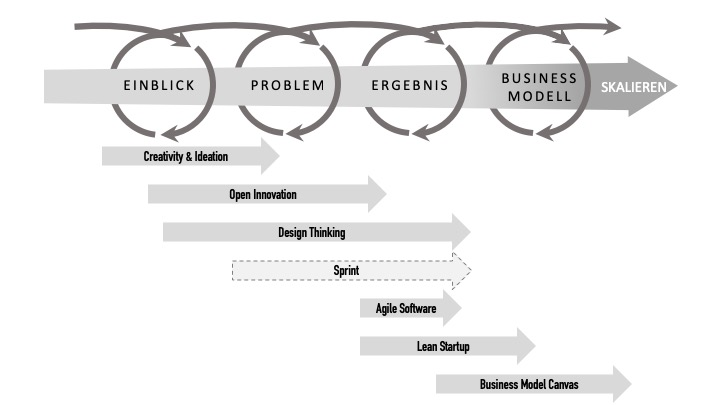
\includegraphics[width=\textwidth]{99_IMG/02_Grundlagen/innovatorsMethod.jpg}
		\caption{The Innovator's Method - Grundkonzept}
		\label{fig:TheInnovatorsMethod}
	\end{center}
\end{figure}

\begin{enumerate}
	\item \textbf{Einblich}
	
	In Schritt 1 liegt der Fokus darauf, die Zielgruppe zu beobachten, zu befragen und kennenzulernen. Erst wenn die Abläufe, welche die potentiellen Kunden zu durchlaufen haben, bekannt sind, kann daran angeknüpft werden. Nicht selten kommt es vor, dass überraschende Details erkannt werden, welche so ursprünglich nicht erwartet wurden. Das sind wesentliche Informationen, die ein kundenorientiertes Konzept ausmachen. Denn nur wenn alle Details über die kritische Ablauffolge klar sind, können daraus resultierende Probleme erkannt werden, wie im nächsten Punkt näher erklärt wird. 
	
	\item \textbf{Problem}
	
	Ein Problem kann hier auch ein Bedürfnis oder einen Wunsch erfüllen. Denn nicht immer löst ein neues Produkt ein bekanntes Problem. Oft werden daher auch Bedürfnisse erfüllt, von welchen der Nutzer ursprünglich nicht wusste, dass er sie hat. Um das herauszufinden, ist es essenziell, Schritt 1 so detailliert durchzuführen, dass diese Wünsche zum Vorschein kommen, ohne dass der Kunde sie formulieren muss. Das Problem per se muss dann gründlich herausgearbeitet werden, indem sich der Gründer in die Lage der Zielgruppe versetzt. Nur so ist es möglich, die entscheidenden Details, welche nicht sofort sichtbar sind, herauszufinden.
	
	\item \textbf{Ergebnis}
	
	Die Lösung des vorher erarbeiteten und untersuchten Problems soll nun prototypisch umgesetzt werden. Im Vergleich zu einem fertig entwickelten Endprodukt hat ein Prototyp viele Vorteile. So kann eine Fassade des Produktes mit minimalem Entwicklungsaufwand ähnliches Feedback erzeugen. Obwohl das Problem vorher bereits eingehend untersucht wird, muss die entwickelte Lösung nicht zwingend optimal sein. Das heißt, die Problematik ist bekannt, allerdings muss das optimale Konzept, diese zu lösen, erst erarbeitet werden. Dazu ist es ineffizient, ein vollständiges Produkt zu entwickeln, denn zuerst muss das Grundkonzept getestet werden, statt den Details. Dafür ist es ohnehin besser, dem Endnutzer einen Prototypen zur Verfügung zu stellen, damit dieser sich nicht in Einzelheiten verlieren kann. Außerdem ist der emotionale Wert des Produktes höher, wenn in dieses bereits viel Zeit investiert wurde. Nachdem das Konzept unter Umständen im Test durchfallen kann und neu entwickelt werden muss, soll dies vermieden werden. Zusammenfassend sollen daher Prototypen von den Endnutzern validiert werden, um die optimale Lösungsstrategie herauszufinden und auf den Kunden abzustimmen. Dieser bestimmt letztendlich den Markterfolg.
	
	\item \textbf{Business Modell}
	
	Erst nachdem bekannt ist, was der Endkunde braucht und wie dieser Wunsch erfüllt werden kann, wird die Marktstrategie erarbeitet. Das gesammelte Wissen über die Zielgruppe ist hier erneut sehr wichtig. Denn ein Produkt, welches zwar optimal auf den Kunden abgestimmt ist, ist nicht wertbringend, wenn die Zielgruppe nicht weiß, dass dieses Produkt exisitert. Daher muss der ideale Weg gefunden werden, die Ware an den Kunden zu bringen. 
\end{enumerate}

Für jeden dieser Schritte sind unter Umständen mehrere Anläufe nötig. Selten schafft es ein Team, die bestmöglichen Ergebnisse in einer Iteration zu erzielen. Doch auch fehlgeschlagene Anläufe sind wertvoll, da das Team aus Irrtümern wiederum wichtige Einblicke in die Kundensicht erlangt. 
\cite{TheInnovatorsMethod}
\newpage 